\documentclass[9pt]{beamer}
\usetheme{Boadilla}
\usepackage{tikz}
 \usepackage[english]{babel}
 \usepackage{amsmath}
 \usepackage{amsfonts}
 \usepackage{amssymb}
 \usepackage{amsthm}
 \usepackage{array}
 \newcommand{\tabitem}{%
  \usebeamertemplate{itemize item}\hspace*{\labelsep}}
 \usepackage{mathtools}
 \DeclarePairedDelimiterX{\inp}[2]{\langle}{\rangle}{#1, #2}
 \usepackage[utf8]{inputenc}
 \usepackage{dsfont}
 \usetikzlibrary{patterns}
 \usepackage{graphicx}
 \graphicspath{{"../Output/"}}
 \usepackage[export]{adjustbox}
 \usepackage{mathrsfs}
 \usepackage{bbold}
\usetikzlibrary{mindmap,trees,shadows}
\usepackage{caption}
\usepackage{tabularx}
\usepackage{booktabs}
\usepackage{caption}
\usepackage{changepage}
\usepackage{subcaption}
\usepackage{import}
\usepackage{hyperref}
% \usepackage{apacite}
\usepackage{listings}
\captionsetup[figure]{font=scriptsize}
\newcommand{\MYhref}[3][blue]{\href{#2}{\color{#1}{#3}}}%
\usepackage{hyperref} 
            \hypersetup{backref=true,       
                    pagebackref=true,               
                    hyperindex=true,                
                    colorlinks=true,                
                    breaklinks=true,                
                    urlcolor= blue,                
                    linkcolor= blue,                
                    bookmarks=true,                 
                    bookmarksopen=false,
                    citecolor=blue,
                    linkcolor=blue,
                    filecolor=blue,
                    citecolor=blue,
                    linkbordercolor=blue
}


\makeatletter
\def\input@path{{"../Output/"}}
\makeatother

\usepackage{biblatex}
\bibliography{References.bib}

\title{M2 Masters Thesis}
\subtitle{Returns Data Summary}
\author{Andrew Boomer}
\date{\today}

\begin{document}

\frame{\titlepage}

\begin{frame}
\begin{itemize}
    \item The S\&P500 monthly data was downloaded from Shiller \href{http://www.econ.yale.edu/~shiller/data.htm}{Data Link}
    \item Data spans monthly from January, 1950 to May 2021, an extension on top of \cite{faias2017optimal}.
    \item The S\&P Composite price is used to calculate log returns ($y_{t}$).
    \item $y_{t}$ are calculated as $y_{t} = ln(S_{t}) - ln(S_{t - 1})$, where $S_{t}$ is the monthly underlying S\&P500 price.
\end{itemize}
\end{frame}

\begin{frame}{GARCH Estimation}
\begin{itemize}
    \item The GARCH(1, 1) model is estimated using data from 1950-2018 inclusive.
    \item The estimation is on $y_{t}$, and is done using maximum likelihood.
    \item We consider a zero-conditional mean specification.
\end{itemize}

The GARCH equation used in the python package is choice B in your slides:

\begin{align}
\nonumber y_{t} &= \sigma_{t} \epsilon_{t} \quad \epsilon_{t} \sim iid.N(0, 1)
\\ \nonumber \sigma_{t}^{2} &= \omega + \alpha y_{t - 1}^{2} + \beta \sigma_{t - 1}^{2}
\end{align}

\[\omega > 0 \ \ \alpha, \beta \geq 0\]
\end{frame}

\begin{frame}{GARCH Estimation}
\begin{center}
\begin{tabular}{lcccc}
    & \textbf{coef} & \textbf{std err} & \textbf{t} & \textbf{P$>|$t$|$} \\
\midrule
$\mathbf{\omega}$ & 0.000 & 0.000 & 3.508 & 0.000 \\
$\mathbf{\alpha}$ & 0.125 & 0.038 & 3.309 & 0.001 \\
$\mathbf{\beta}$ & 0.783 & 0.037 & 21.404 & 0.000 \\
\bottomrule
\end{tabular}
\end{center}
\end{frame}

\begin{frame}{GARCH Estimation}
\framesubtitle{GARCH Time Series Plot}
\begin{center}
	\begin{figure}
		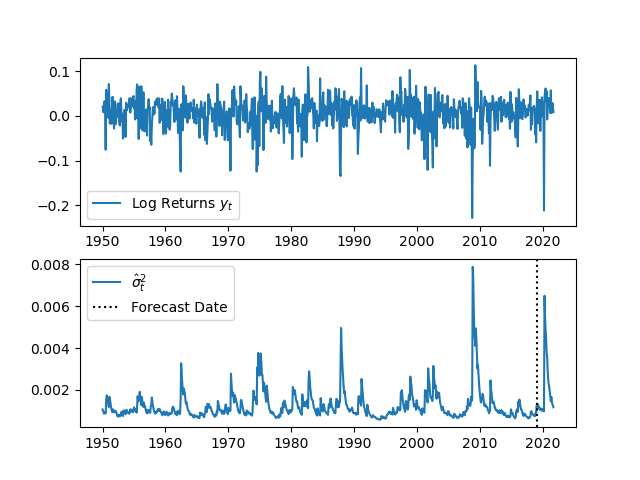
\includegraphics[width=9cm]{GARCH_TS_plot.png}
	\end{figure}
\end{center}
\end{frame}

\begin{frame}{Replication of Table 1 \citeauthor{faias2017optimal}}
\begin{itemize}
    \item Standardized Returns ($\hat{\epsilon}_{t}$) are calculated using the conditional volatility time series obtained from the GARCH estimation. $\hat{\epsilon}_{t} = \frac{y_{t}}{\hat{\sigma}_{t}^{GARCH}}$
    \item Skew is calculated as $\frac{\frac{1}{N} \sum_{n = 1}^{N} (x_{n} - \bar{x})^{3}}{(\frac{1}{N}\sum_{n = 1}^{N} (x_{n} - \bar{x})^{2})^{\frac{3}{2}}}$
    \item Kurtosis is calculated as $\frac{\frac{1}{N} \sum_{n = 1}^{N} (x_{n} - \bar{x})^{4}}{(\frac{1}{N}\sum_{n = 1}^{N} (x_{n} - \bar{x})^{2})^{2}}$
    \item Lag 1 Autocorrelation is calculated as: $corr(y_{t}, y_{t-1})$ where $L$ is the Lag Operator
    \item Lag 1 Squared Autocorrelation is calculated as: $corr(y_{t}^{2}, y_{t-1}^{2})$
    \item Used Ljung-Box test of autocorrelation with a lag of 1 for $Q_{1}(z)$
    \item For ARCH test, used Engle’s Test for Autoregressive Conditional Heteroscedasticity (ARCH) with lag of 1.
\end{itemize} 
\end{frame}

\begin{frame}
    \begin{center}
        \begin{figure}
            \caption{Table 1}
            \scalebox{0.7}{\begin{tabular}{lccccccc} 
    & \multicolumn{3}{c} { Log Returns $y_{t}$} & & \multicolumn{3}{c} { Standardized Returns $\hat{\epsilon}_{t}$} \\
    \cline { 2 - 4 } \cline { 6 - 8 } Statistics & $1950-2018$ & $2019-2021$ & $1950-2021$ & & $1950-2018$ & $2019-2021$ & $1950-2021$ \\
    \hline

    No. of obs. & 828 & 33 & 861 & & 828 & 33 & 861 \\
    Skewness & $-1.01$ & $-3.7$ & $-1.22$ & & $-0.89$ & $-4.25$ & $-1.2$ \\
    Excess kurtosis & $3.99$ & $15.91$ & $5.12$ & & $2.57$ & $19.52$ & $4.68$ \\
    $\rho_{1}(z)$ & $0.24$ & $-0.02$ & $0.22$ & & $0.18$ & $-0.01$ & $0.17$ \\
    $\rho_{1}\left(z^{2}\right)$ & $0.15$ & $-0.04$ & $0.11$ & & $0.0$ & $-0.06$ & $-0.01$ \\
    $Q_{1}(z)$ & $46.52$ & $0.01$ & $42.55$ & & $28.34$ & $0.0$ & $25.32$ \\
    & {$[0.0]$} & {$[0.9]$} & {$[0.0]$} & & {$[0.0]$} & {$[0.96]$} & {$[0.0]$} \\
    ARCH(1) & $19.35$ & $0.06$ & $10.74$ & & $0.02$ & $0.09$ & $0.15$ \\
    & {$[0.0]$} & {$[0.81]$} & {$[0.0]$} & & {$[0.9]$} & {$[0.76]$} & {$[0.7]$} \\
    \hline
    \end{tabular}}
        \end{figure}
    \end{center}
\end{frame}

\begin{frame}{Volatility Forecast}
\begin{itemize}
    \item Volatility forecasts are computed for the time period of 2019-May 2021 inclusive.
    \item The volatility forecast at time $t + h$ uses the information of the actual $y_{t}$ at time $t + h - 1$.
    \item This is done under a fixed estimation window scheme, where the GARCH model parameters are only estimated once. If time allows, a rolling estimation window will be employed where the GARCH parameters are re-estimated at each time period.
\end{itemize}

For each time period $t + h$ beginning in January 2019, the variance forecast is:

\[\hat{\sigma}_{t + h}^{2} = \hat{\omega} + \hat{\alpha} y_{t + h - 1}^{2} + \hat{\beta} \hat{\sigma}_{t + h - 1}^{2}\]

The volatility is then $\hat{\sigma}_{t + h} = \sqrt{\hat{\sigma}_{t + h}^{2}}$
\end{frame}

\begin{frame}{Historic Standardized Return}
\begin{center}
\begin{figure}
    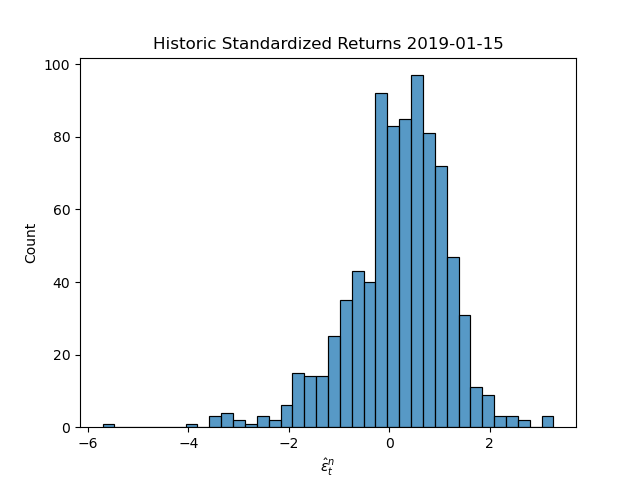
\includegraphics[width=9cm]{SR_20190115.png}
\end{figure}
\end{center}
\end{frame}

\begin{frame}{Historic Log Returns}
\begin{center}
\begin{figure}
    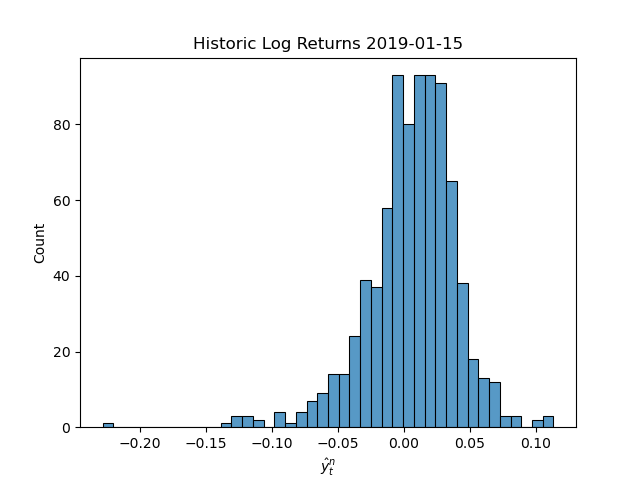
\includegraphics[width=9cm]{RR_20190115.png}
\end{figure}
\end{center}
\end{frame}

\begin{frame}{Step 1: \citeauthor{faias2017optimal}}
\framesubtitle{Bootstrap $y_{t}$ Simulation}
\begin{itemize}
    \item To simulate log returns, first the $\epsilon_{t}$ are simulated ($\tilde{\epsilon}_{t}$) using a bootstrapping method from historical $\hat{\epsilon}_{t}$. This follows the filtered historical simulation method in \citeauthor{barone2008garch}.
    \item At each time t beginning January 2019, N samples are chosen with replacement from the historical $\hat{\epsilon}_{t}$ series, time t inclusive.
    \item With 29 months between January 2019 and May 2021, this gives a bootsrapped matrix of $\tilde{\epsilon}_{t}$ of size $29 \times N$.
    \item The volatility forecast time series is then multiplied by each of the N simulation for each of the time periods such that $y_{t + h}^{n} = \hat{\sigma}_{t + h} \tilde{\epsilon}_{t + h}^{n} \quad \forall n \in 1, \dotsb, N$
    \item The result is a matrix of simulated $y_{t}$.
\end{itemize}
\end{frame}

\begin{frame}{Step 2: \citeauthor{faias2017optimal}}
\framesubtitle{Underlying Price Simulation}
For each period $t + h$ starting January 2019, and for each simulation $n \in N$, the simulated price is calculated as:

\[S_{t + h|t+h-1}^{n} = S_{t + h - 1} e^{y_{t + h}^{n}}\]

This yields a matrix of simulated asset prices with an equivalent shape to the matrix of $y_{t}$.
\end{frame}

\begin{frame}{Option Data}
The option data for the SP500 index (SPX) was provided from the CBOE.

\begin{center}
	\begin{tabular}{ll}
\hline
 Variable Name     & Description              \\
\hline
 underlying\_symbol & Asset Symbol             \\
 quote\_date        & Quote Time               \\
 expiration        & Contract Expiration Date \\
 strike            & Contract Strike Price    \\
 option\_type       & Contract Type: Call/Put  \\
 open              & Option Price at Open     \\
 close             & Option Price at Close    \\
 high              & High Option Price        \\
 low               & Low Option Price         \\
 Volume            & Contract Trading Volume  \\
\hline
\end{tabular}
\end{center}
\end{frame}

\begin{frame}{Option Data}
\begin{center}
	\begin{figure}
		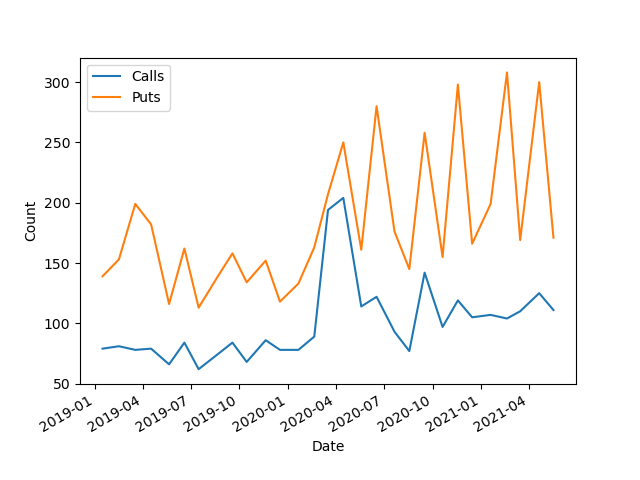
\includegraphics[width=9cm]{Contract_Count.png}
	\end{figure}
\end{center}
\end{frame}

\begin{frame}{Option Data}
\framesubtitle{Cleaning the Data}
\begin{itemize}
    \item Following \citeauthor{faias2017optimal}, observations are filtered for 3 criteria: Zero Volume Traded, Bid Price lower than $\$0.125$, and Bid Price lower than Ask Price. Arbitrage bound violation has not been filtered.
    \item These 3 filters correspond to the columns: 'Volume', 'bid\_eod', and 'ask\_eod' respectively.
    \item The data is then filtered for expiration dates that land on the 3rd Friday of each month. 
    \item Then option quote times are filtered for 1 month to maturity, 28/29/30/31 days depending on the month and year.
\end{itemize}
\end{frame}

\begin{frame}{Risk Free Asset}
\begin{itemize}
    \item As in \citeauthor{faias2017optimal}, the 1-month treasury bill time series is used as the risk free asset.
    \item The daily data is downloaded from the FRED website here \href{https://fred.stlouisfed.org/series/DGS1MO}{TBill Link}
    \item This data is then joined to match up with the quote time of the options in the filtered CBOE data.
    \item This produces a time series of risk free returns, that as in \citeauthor{faias2017optimal}, we take as given.
\end{itemize}
\end{frame}

\begin{frame}{Step 3: \citeauthor{faias2017optimal}}
\framesubtitle{Simulated Option Returns}
The option returns are calculated assuming the contract is held until expiration.
This means that the simulated payoff of a call and a put respectively are:

\[C_{t+1|t}^{n} = max(S_{t+1|t}^{n} - K_{t, c}, 0)\]
\[P_{t+1|t}^{n} = max(K_{t, p} - S_{t+1|t}^{n}, 0)\]

\[\forall \ n \in N\]

Where $K_{t, c}$ and $K_{t, p}$ and the strike prices for the respective call and put contracts.

The simulated returns are then:
\[r_{t+1|t, c}^{n} = \frac{C_{t+1|t}^{n}}{C_{t, c}} - 1 \quad \text{and} \quad r_{t+1|t, p}^{n} = \frac{P_{t+1|t}^{n}}{P_{t, p}} - 1\]

$C_{t, c}$ and $P_{t, p}$ is using the closing price from the CBOE data.
\end{frame}

\begin{frame}{Step 4: \citeauthor{faias2017optimal}}
\framesubtitle{Simulated Returns}
\citeauthor{faias2017optimal} present the simulated portfolio returns for a simulation $n$ as:

\[rp_{t+1 \mid t}^{n} = rf_{t}+\sum_{c = 1}^{C} \omega_{t, c}\left(r_{t + 1 \mid t, c}^{n} - rf_{t}\right)+\sum_{p = 1}^{P} \omega_{t, p}\left(r_{t + 1 \mid t, p}^{n} - rf_{t}\right)\]

Where $rf_{t}$ is the risk free rate, represented by the 1 month Treasury Bill time series.

In terms of implementation, this can be vectorized be concatenating the call and put returns, as well as the call and put weights to get:

\[rp_{t+1 \mid t}^{n} = rf_{t} + \inp{\mathbf{W}_{t, cp}}{\mathbf{R_{t+1|t, cp}^{n}}}\]

Where $\mathbf{W}_{t, cp} = \begin{bmatrix} \omega_{t, c_{1}}, \dotsb, \omega_{t, c_{C}}, \omega_{t, p_{1}}, \dotsb, \omega_{t, p_{P}} \end{bmatrix}$ \\
and \\
$\mathbf{R}_{t+1|t, cp}^{n} = \begin{bmatrix} r_{t + 1|t, c_{1}}^{n}, \dotsb, r_{t + 1|t, c_{C}}^{n}, r_{t + 1|t, p_{1}}^{n}, \dotsb, r_{t + 1|t, p_{P}}^{n} \end{bmatrix} - \begin{bmatrix} rf_{t}, \dotsb, rf_{t} \end{bmatrix}$
\end{frame}

\begin{frame}{Step 5: \citeauthor{faias2017optimal}}
\framesubtitle{Expected Utility Optimization}
\citeauthor{faias2017optimal} present a power utility function to use for the optimization. This function has the property of constant relative risk aversion (CRRA). \citeauthor{faias2017optimal} mention that previous literature has estimated $\gamma$ as 4, but they use a value of 10, which I follow.

\[U(W)=\left\{\begin{array}{ll}\frac{1}{1-\gamma} W^{1-\gamma}, & \text { if } \gamma \neq 1 \\ \ln (W), & \text { if } \gamma=1\end{array}\right.\]

% They additioanlly argue that the optimization at time $t$ is independent of the current wealth $W_{t}$, so that:
% \[E[U(W_{t}(1 + rp^{n}_{t+1|t}))] = E[U((1 + rp^{n}_{t+1|t}))]\]

\citeauthor{faias2017optimal} go through a derivation to get a simplified maximization problem in this setting. In terms of the vectorized implementation, across all $N$ simulations, we maximize mean utility:

\[\underset{\mathbf{W}_{t, cp}}{max} \sum_{n = 1}^{N} U(1 + rp_{t+1 \mid t}^{n})\]

From this optimization, we get a set of weights.
\end{frame}

\begin{frame}{Step 6, 7, 8: \citeauthor{faias2017optimal}}
\framesubtitle{Out of Sample Returns}
\begin{itemize}
    \item The ex-post returns $rp_{t+1}$ are calculated with the same procedure as the simulated returns.
    \item The true underlying asset price at $t+1$, $S_{t+1}$ is used in place of the simulated one $S_{t+1|t}^{n}$
\end{itemize}

\begin{align}
\nonumber C_{t+1} &= max(S_{t+1} - K_{t, c}, 0), \quad P_{t+1} = max(K_{t, p} - S_{t+1}, 0)
\\ \nonumber r_{t+1, c} &= \frac{C_{t+1}}{C_{t, c}} - 1 \quad \text{and} \quad r_{t+1, p} = \frac{P_{t+1}}{P_{t, p}} - 1
\\ \nonumber \text{Which gives } & \mathbf{R}_{t+1, cp} = \begin{bmatrix} r_{t + 1, c_{1}}, \dotsb, r_{t + 1, c_{C}}, r_{t + 1, p_{1}}, \dotsb, r_{t + 1, p_{P}} \end{bmatrix} - \begin{bmatrix} rf_{t}, \dotsb, rf_{t} \end{bmatrix}
\\ \nonumber \mathbf{W}_{t, cp} & \text{ is obtained from Step 5 optimization}
\end{align}

\[rp_{t+1} = rf_{t} + \inp{\mathbf{W}_{t, cp}}{\mathbf{R_{t+1, cp}}}\]

Next periods wealth is:

\[W_{t+1} = W_{t} (1 + rp_{t+1})\]
\end{frame}

\begin{frame}{Optimization Implementation}
\begin{itemize}
    \item I have implemented a partial version of their optimization, and gotten some results. There appears to be something not quite right. I will look into potential issues.
    \item In order to take transaction costs into account, they duplicate each option contract for a short/long position with bid/ask prices. The short contracts enter with the negative of the return.
    \item Additionally, I have included two optimization scenarios, one where only the four contracts in \citeauthor{faias2017optimal} are included, and one where all available contracts are included. Results are presented for each.
\end{itemize}
\end{frame}

\begin{frame}{Monthly Returns Sample}
\framesubtitle{Optimization with 4 Contracts}
\begin{columns}
    \column{0.5\textwidth}
    \begin{center}
    \scalebox{0.6}{\begin{tabular}{llrrrrrr}
\hline
 Date       & Expiry     &   ExPost &   ATM\_Call\_Weight &   OTM\_Call\_Weight &   ATM\_Put\_Weight &   OTM\_Put\_Weight &   RfWeight \\
\hline
 2019-01-15 & 2019-02-15 &    -6.3\% &             -4.0\% &              0.6\% &             2.6\% &            -2.6\% &     103.3\% \\
 2019-02-15 & 2019-03-15 &    -3.0\% &             -7.5\% &             -0.7\% &            11.3\% &            -4.6\% &     101.6\% \\
 2019-03-18 & 2019-04-18 &    -5.8\% &             -7.5\% &              1.0\% &             2.9\% &            -1.8\% &     105.5\% \\
 2019-04-17 & 2019-05-17 &    10.5\% &             -5.0\% &              1.3\% &             6.5\% &            -1.9\% &      99.2\% \\
 2019-05-21 & 2019-06-21 &     2.8\% &              1.9\% &              0.3\% &            -1.8\% &             0.0\% &      99.5\% \\
 2019-06-19 & 2019-07-19 &    -5.2\% &             -9.6\% &              1.2\% &             0.9\% &            -0.8\% &     108.3\% \\
 2019-07-16 & 2019-08-16 &    22.9\% &             -8.1\% &              1.1\% &             5.7\% &            -2.4\% &     103.7\% \\
 2019-08-20 & 2019-09-20 &     4.5\% &              3.1\% &              1.4\% &            -1.2\% &            -1.2\% &      97.9\% \\
 2019-09-18 & 2019-10-18 &    11.5\% &            -12.4\% &              1.6\% &             5.5\% &            -3.9\% &     109.3\% \\
 2019-10-15 & 2019-11-15 &    -1.9\% &             -2.6\% &              0.4\% &            -0.3\% &            -0.5\% &     103.0\% \\
 2019-11-20 & 2019-12-20 &   -12.2\% &            -12.0\% &              1.1\% &             6.7\% &            -3.2\% &     107.5\% \\
 2019-12-17 & 2020-01-17 &    -7.7\% &             -5.7\% &              0.5\% &             4.0\% &            -2.3\% &     103.5\% \\
 2020-01-21 & 2020-02-21 &    18.1\% &            -19.2\% &              1.4\% &             3.3\% &            -1.9\% &     116.4\% \\
 2020-02-20 & 2020-03-20 &    -7.7\% &            -43.8\% &              3.9\% &            -5.6\% &             2.1\% &     143.3\% \\
 2020-03-17 & 2020-04-17 &   603.3\% &             -2.0\% &              0.7\% &          -602.9\% &             0.0\% &     704.2\% \\
 2020-04-15 & 2020-05-15 &    -3.4\% &            -10.6\% &              3.5\% &             2.8\% &            -3.6\% &     108.0\% \\
 2020-05-19 & 2020-06-19 &    -5.2\% &             -2.2\% &              0.2\% &            19.5\% &           -16.7\% &      99.1\% \\
 2020-06-17 & 2020-07-17 &    -4.7\% &            -12.9\% &              3.4\% &            13.0\% &           -11.1\% &     107.5\% \\
 2020-07-21 & 2020-08-21 &    -6.6\% &             -8.4\% &              3.2\% &             3.1\% &            -2.2\% &     104.2\% \\
 2020-08-18 & 2020-09-18 &     2.2\% &             -6.4\% &              1.1\% &             7.8\% &            -4.6\% &     102.1\% \\
 2020-09-16 & 2020-10-16 &     0.7\% &             -5.2\% &              2.6\% &             2.7\% &            -2.9\% &     102.8\% \\
 2020-10-20 & 2020-11-20 &    -0.5\% &             -7.6\% &              1.1\% &             3.2\% &            -4.2\% &     107.5\% \\
 2020-11-18 & 2020-12-18 &   -10.5\% &            -13.4\% &              4.8\% &            10.9\% &            -9.2\% &     106.9\% \\
 2020-12-15 & 2021-01-15 &    -3.4\% &             -2.2\% &             -0.7\% &             9.1\% &            -6.4\% &     100.1\% \\
 2021-01-19 & 2021-02-19 &    -2.0\% &             -7.0\% &              0.8\% &             4.5\% &            -4.1\% &     105.8\% \\
 2021-02-19 & 2021-03-19 &     6.6\% &            -11.0\% &              4.3\% &             3.0\% &            -2.9\% &     106.6\% \\
 2021-03-16 & 2021-04-16 &    -5.9\% &             -6.1\% &              0.5\% &             1.8\% &            -1.8\% &     105.6\% \\
 2021-04-21 & 2021-05-21 &     3.6\% &            -11.2\% &              1.8\% &            12.7\% &            -6.9\% &     103.6\% \\
 2021-05-18 & 2021-06-18 &     1.6\% &             -1.7\% &              0.3\% &            -1.1\% &            -0.7\% &     103.2\% \\
\hline
\end{tabular}}
    \end{center}
    \column{0.5\textwidth}
    \begin{itemize}
        \item Using OTM/ATM Call/Put as in \citeauthor{faias2017optimal}. Returns appear reasonable
        \item Sharpe Ratio of $\sim 0.18$
    \end{itemize}
\end{columns}
\end{frame}

% \begin{frame}{Monthly Returns Sample}
% \framesubtitle{Optimization with all Contracts}
% \begin{columns}
%     \column{0.5\textwidth}
%     \begin{center}
%     \scalebox{0.6}{\begin{tabular}{llr}
\toprule
      Date &     Expiry &  rp\_t+1 \\
\midrule
2019-01-15 & 2019-02-15 &   11.41 \\
2019-02-15 & 2019-03-15 &   18.10 \\
2019-03-18 & 2019-04-18 &   19.38 \\
2019-04-17 & 2019-05-17 &   36.51 \\
2019-05-21 & 2019-06-21 &   15.58 \\
2019-06-19 & 2019-07-19 &   12.17 \\
2019-07-16 & 2019-08-16 &   20.09 \\
2019-08-20 & 2019-09-20 &   13.96 \\
2019-09-18 & 2019-10-18 &   14.54 \\
2019-10-15 & 2019-11-15 &   12.24 \\
2019-11-20 & 2019-12-20 &   28.15 \\
2019-12-17 & 2020-01-17 &   15.60 \\
2020-01-21 & 2020-02-21 &   13.90 \\
2020-02-20 & 2020-03-20 & -145.33 \\
2020-03-17 & 2020-04-17 &   10.62 \\
2020-04-15 & 2020-05-15 &   16.25 \\
2020-05-19 & 2020-06-19 &   16.30 \\
2020-06-17 & 2020-07-17 &   13.93 \\
2020-07-21 & 2020-08-21 &   22.11 \\
2020-08-18 & 2020-09-18 &   19.86 \\
2020-09-16 & 2020-10-16 &   21.15 \\
2020-10-20 & 2020-11-20 &   11.73 \\
2020-11-18 & 2020-12-18 &   27.06 \\
2020-12-15 & 2021-01-15 &   14.84 \\
2021-01-19 & 2021-02-19 &   14.02 \\
2021-02-19 & 2021-03-19 &   17.32 \\
2021-03-16 & 2021-04-16 &   15.35 \\
2021-04-21 & 2021-05-21 &   19.21 \\
2021-05-18 & 2021-06-18 &   17.81 \\
\bottomrule
\end{tabular}}
%     \end{center}
%     \column{0.5\textwidth}
%     \begin{itemize}
%         \item Sharpe ratio of $\sim 0.39$
%         \item The total sum of the weights put into short contracts is roughly 3.5 times greater than the amount into long ones.
%         \item The mean of the sum of the weights per Date is $\sim -17.12$
%     \end{itemize}
% \end{columns}
% \end{frame}

\begin{frame}{Weights Plot \citeauthor{faias2017optimal}}
\begin{columns}
\column{0.7\textwidth}
\begin{figure}
    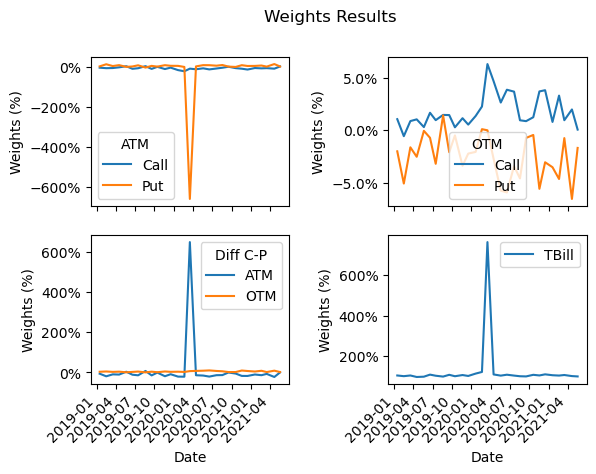
\includegraphics[width=8cm]{WeightsPlot.png}
\end{figure}
\column{0.45\textwidth}
\begin{center}
\begin{itemize}
    \item  
\end{itemize}
\end{center}
\end{columns}
\end{frame}

\begin{frame}{Density of Returns by Contract Type}
\begin{columns}
\column{0.7\textwidth}
\begin{figure}
    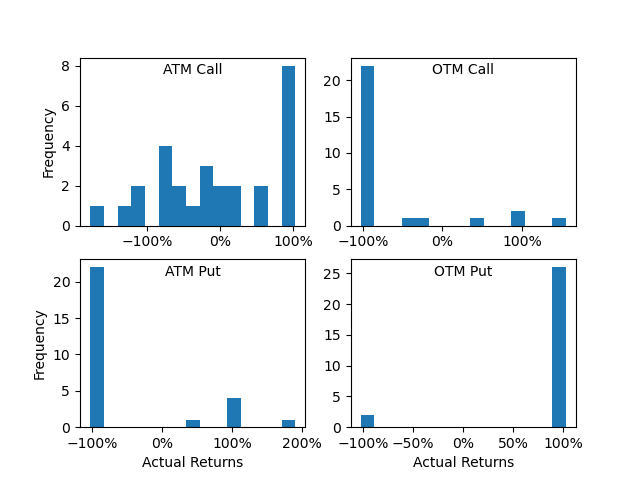
\includegraphics[width=8cm]{Fig3_kde.png}
\end{figure}
\column{0.45\textwidth}
\begin{center}
\begin{itemize}
    \item  
\end{itemize}
\end{center}
\end{columns}
\end{frame}

\begin{frame}{Density of Optimization Returns}
\begin{columns}
\column{0.7\textwidth}
\begin{figure}
    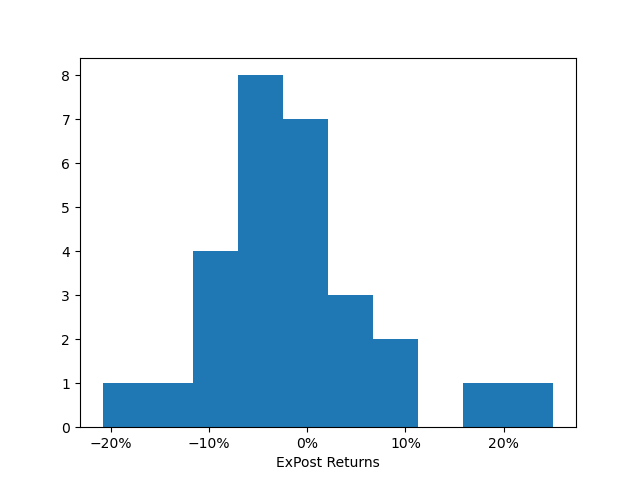
\includegraphics[width=8cm]{Fig4_OOPSRet.png}
\end{figure}
\column{0.45\textwidth}
\begin{center}
\begin{itemize}
    \item  
\end{itemize}
\end{center}
\end{columns}
\end{frame}

\begin{frame}{Optimization Returns Summary}
\framesubtitle{Individual Option Types}
\begin{center}
	\begin{tabular}{lrrrrrrr}
\hline
                &   Mean &     Std &     Min &     Max &   Skew &   Kurtosis &    SR \\
\hline
 ATM\_Call       &  13.5\% &   98.3\% & -100.0\% &  298.3\% &   0.71 &       0.49 &  0.14 \\
 ATM\_Put        &  19.3\% &  561.8\% & -100.0\% & 2923.5\% &   5.01 &      23.42 &  0.03 \\
 OTM\_Call       & -55.2\% &  122.9\% & -100.0\% &  498.1\% &   3.53 &      12.62 & -0.45 \\
 OTM\_Put        &  89.1\% & 1018.2\% & -100.0\% & 5383.4\% &   5.10 &      24.04 &  0.09 \\
 1/N rule       & -19.6\% &  107.8\% & -100.0\% &  480.8\% &   3.58 &      14.29 & -0.18 \\
 S\&P 500        &   1.8\% &    4.7\% &  -19.1\% &    6.3\% &  -3.14 &      11.59 &  0.38 \\
 1-month T-bill & -14.2\% &   31.6\% & -100.0\% &   44.4\% &  -1.34 &       1.66 & -0.45 \\
\hline
\end{tabular}
\end{center}
\end{frame}

\begin{frame}{Optimization Returns Summary}
\framesubtitle{Optimizer vs. S\&P 500}
\begin{center}
	\begin{tabular}{lrrrrrrr}
\hline
         &   Mean &   Std &   Min &   Max &   Skew &   Kurtosis &   SR \\
\hline
 S\&P 500 &    1.8 &   4.7 & -19.1 &   6.3 &  -3.14 &      11.59 & 0.38 \\
 ExPost  &    0.7 &   5.0 & -19.9 &  11.5 &  -2.22 &       9.15 & 0.15 \\
\hline
\end{tabular}
\end{center}
\end{frame}

\begin{frame}{Optimization Weights Summary}
\begin{center}
	\begin{tabular}{lrrrr}
\hline
         &   ATM Call &   ATM Put &   OTM Call &   OTM Put \\
\hline
 Mean    &       -2.4 &      -0.0 &        0.5 &      -1.1 \\
 Minimum &      -25.4 &      -3.0 &       -1.9 &      -9.5 \\
 Maximum &        1.7 &       2.9 &        2.1 &       0.3 \\
\hline
\end{tabular}
\end{center}
\end{frame}

% \begin{frame}{1 Month Treasury Bill Plot}
% \begin{columns}
% \column{0.5\textwidth}
% \begin{figure}
%     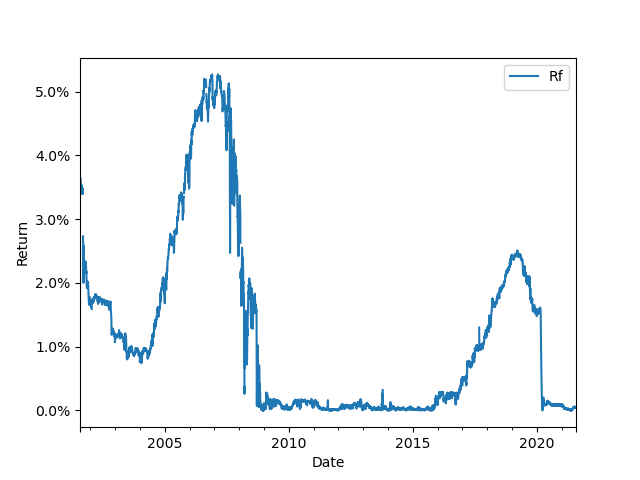
\includegraphics[width=6cm]{Tbill_TS.png}
% \end{figure}
% \column{0.45\textwidth}
% \begin{center}
% \begin{itemize}
%     \item The only positive return from the sample in the previous slide correpsonds to the crash in the 1 month tbill rate at the beginning of COVID. 
% \end{itemize}
% \end{center}
% \end{columns}
% \end{frame}

% \begin{frame}{Introduction}
% \framesubtitle{Introduction}
% \begin{itemize}
%     \item This presentation is an attempt to show the progress I have made towards the implementation of the project that I have made so far.
%     \item Since this implementation has taken most of my time, I haven't been able to go more deeply into the optimization theory to understand which algorithms/solvers I should be using in my context.
%     \item Because of this, I do{}n't have a very detailed explanation of how the solvers I am currently using work. But depending on what you think the best use of my time is, I can dive into this in more detail and understand this portion better.
% \end{itemize}
% \end{frame}

% \begin{frame}{Overview}
% \framesubtitle{Implementation Flow Chart}
% \begin{center}
%     \scalebox{0.65}{

\tikzset{every picture/.style={line width=0.75pt}} %set default line width to 0.75pt        

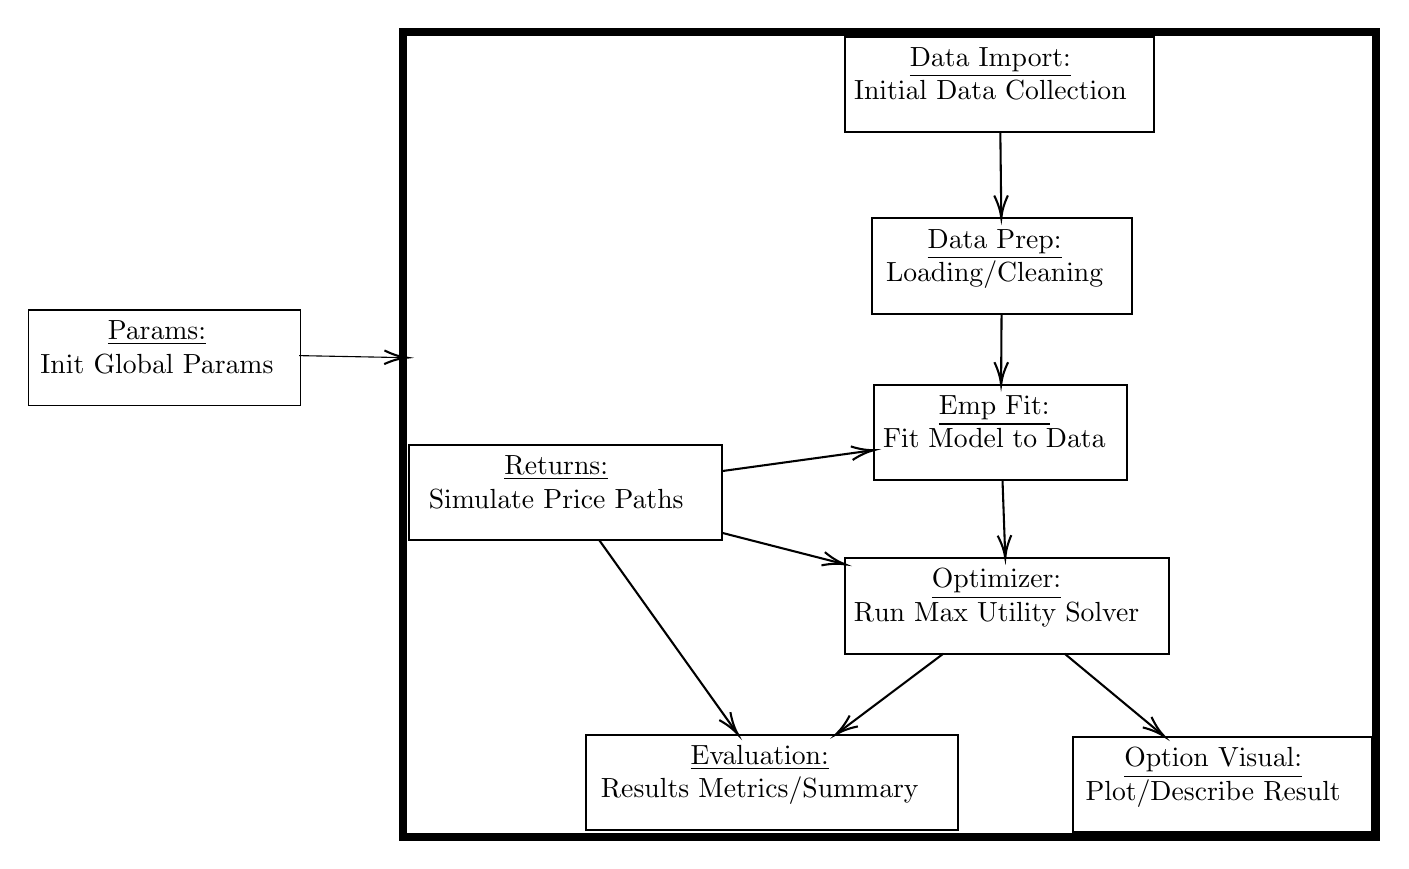
\begin{tikzpicture}[x=0.75pt,y=0.75pt,yscale=-1,xscale=1]
%uncomment if require: \path (0,549); %set diagram left start at 0, and has height of 549

%Shape: Rectangle [id:dp641267805615122] 
\draw  [line width=3]  (192.5,56) -- (661.5,56) -- (661.5,444) -- (192.5,444) -- cycle ;

%Straight Lines [id:da14098325743213436] 
\draw    (142.5,212) -- (192.5,212.96) ;
\draw [shift={(194.5,213)}, rotate = 181.1] [color={rgb, 255:red, 0; green, 0; blue, 0 }  ][line width=0.75]    (10.93,-3.29) .. controls (6.95,-1.4) and (3.31,-0.3) .. (0,0) .. controls (3.31,0.3) and (6.95,1.4) .. (10.93,3.29)   ;

% Text Node
\draw    (12,190) -- (143,190) -- (143,236) -- (12,236) -- cycle  ;
\draw (15,194) node [anchor=north west][inner sep=0.75pt]   [align=left] {\begin{minipage}[lt]{86.63pt}\setlength\topsep{0pt}
\begin{center}
\underline{Params:}\\Init Global Params
\end{center}

\end{minipage}};
% Text Node
\draw  [color={rgb, 255:red, 0; green, 0; blue, 0 }  ,draw opacity=1 ][line width=0.75]   (405.6,58.41) -- (554.6,58.41) -- (554.6,104.41) -- (405.6,104.41) -- cycle  ;
\draw (408.6,62.41) node [anchor=north west][inner sep=0.75pt]   [align=left] {\begin{minipage}[lt]{98.54pt}\setlength\topsep{0pt}
\begin{center}
\underline{Data Import:}\\Initial Data Collection
\end{center}

\end{minipage}};
% Text Node
\draw  [color={rgb, 255:red, 0; green, 0; blue, 0 }  ,draw opacity=1 ][line width=0.75]   (418.59,145.8) -- (543.59,145.8) -- (543.59,191.8) -- (418.59,191.8) -- cycle  ;
\draw (421.59,149.8) node [anchor=north west][inner sep=0.75pt]   [align=left] {\begin{minipage}[lt]{82.12pt}\setlength\topsep{0pt}
\begin{center}
\underline{Data Prep:}\\Loading/Cleaning
\end{center}

\end{minipage}};
% Text Node
\draw  [color={rgb, 255:red, 0; green, 0; blue, 0 }  ,draw opacity=1 ][line width=0.75]   (419.59,226.11) -- (541.59,226.11) -- (541.59,272.11) -- (419.59,272.11) -- cycle  ;
\draw (422.59,230.11) node [anchor=north west][inner sep=0.75pt]   [align=left] {\begin{minipage}[lt]{80.39pt}\setlength\topsep{0pt}
\begin{center}
\underline{Emp Fit:}\\Fit Model to Data
\end{center}

\end{minipage}};
% Text Node
\draw  [color={rgb, 255:red, 0; green, 0; blue, 0 }  ,draw opacity=1 ][line width=0.75]   (280.9,394.59) -- (459.9,394.59) -- (459.9,440.59) -- (280.9,440.59) -- cycle  ;
\draw (283.9,398.59) node [anchor=north west][inner sep=0.75pt]   [align=left] {\begin{minipage}[lt]{118.9pt}\setlength\topsep{0pt}
\begin{center}
\underline{Evaluation:}\\Results Metrics/Summary
\end{center}

\end{minipage}};
% Text Node
\draw  [color={rgb, 255:red, 0; green, 0; blue, 0 }  ,draw opacity=1 ][line width=0.75]   (405.58,309.56) -- (561.58,309.56) -- (561.58,355.56) -- (405.58,355.56) -- cycle  ;
\draw (408.58,313.56) node [anchor=north west][inner sep=0.75pt]   [align=left] {\begin{minipage}[lt]{103.05pt}\setlength\topsep{0pt}
\begin{center}
\underline{Optimizer:}\\Run Max Utility Solver
\end{center}

\end{minipage}};
% Text Node
\draw  [color={rgb, 255:red, 0; green, 0; blue, 0 }  ,draw opacity=1 ][line width=0.75]   (515.2,395.59) -- (659.2,395.59) -- (659.2,441.59) -- (515.2,441.59) -- cycle  ;
\draw (518.2,399.59) node [anchor=north west][inner sep=0.75pt]   [align=left] {\begin{minipage}[lt]{95.13pt}\setlength\topsep{0pt}
\begin{center}
\underline{Option Visual:}\\Plot/Describe Result
\end{center}

\end{minipage}};
% Text Node
\draw  [color={rgb, 255:red, 0; green, 0; blue, 0 }  ,draw opacity=1 ][line width=0.75]   (195.29,255.05) -- (346.29,255.05) -- (346.29,301.05) -- (195.29,301.05) -- cycle  ;
\draw (198.29,259.05) node [anchor=north west][inner sep=0.75pt]   [align=left] {\begin{minipage}[lt]{100.24pt}\setlength\topsep{0pt}
\begin{center}
\underline{Returns:}\\Simulate Price Paths 
\end{center}

\end{minipage}};
% Connection
\draw [color={rgb, 255:red, 0; green, 0; blue, 0 }  ,draw opacity=1 ][line width=0.75]    (480.95,191.8) -- (480.74,224.11) ;
\draw [shift={(480.73,226.11)}, rotate = 270.36] [color={rgb, 255:red, 0; green, 0; blue, 0 }  ,draw opacity=1 ][line width=0.75]    (10.93,-3.29) .. controls (6.95,-1.4) and (3.31,-0.3) .. (0,0) .. controls (3.31,0.3) and (6.95,1.4) .. (10.93,3.29)   ;
% Connection
\draw [color={rgb, 255:red, 0; green, 0; blue, 0 }  ,draw opacity=1 ][line width=0.75]    (481.41,272.11) -- (482.68,307.56) ;
\draw [shift={(482.75,309.56)}, rotate = 267.95] [color={rgb, 255:red, 0; green, 0; blue, 0 }  ,draw opacity=1 ][line width=0.75]    (10.93,-3.29) .. controls (6.95,-1.4) and (3.31,-0.3) .. (0,0) .. controls (3.31,0.3) and (6.95,1.4) .. (10.93,3.29)   ;
% Connection
\draw [color={rgb, 255:red, 0; green, 0; blue, 0 }  ,draw opacity=1 ][line width=0.75]    (346.29,267.63) -- (417.61,257.8) ;
\draw [shift={(419.59,257.52)}, rotate = 532.15] [color={rgb, 255:red, 0; green, 0; blue, 0 }  ,draw opacity=1 ][line width=0.75]    (10.93,-3.29) .. controls (6.95,-1.4) and (3.31,-0.3) .. (0,0) .. controls (3.31,0.3) and (6.95,1.4) .. (10.93,3.29)   ;
% Connection
\draw [color={rgb, 255:red, 0; green, 0; blue, 0 }  ,draw opacity=1 ][line width=0.75]    (346.29,297.39) -- (403.64,312.08) ;
\draw [shift={(405.58,312.58)}, rotate = 194.37] [color={rgb, 255:red, 0; green, 0; blue, 0 }  ,draw opacity=1 ][line width=0.75]    (10.93,-3.29) .. controls (6.95,-1.4) and (3.31,-0.3) .. (0,0) .. controls (3.31,0.3) and (6.95,1.4) .. (10.93,3.29)   ;
% Connection
\draw [color={rgb, 255:red, 0; green, 0; blue, 0 }  ,draw opacity=1 ][line width=0.75]    (452.96,355.56) -- (402.61,393.39) ;
\draw [shift={(401.01,394.59)}, rotate = 323.08000000000004] [color={rgb, 255:red, 0; green, 0; blue, 0 }  ,draw opacity=1 ][line width=0.75]    (10.93,-3.29) .. controls (6.95,-1.4) and (3.31,-0.3) .. (0,0) .. controls (3.31,0.3) and (6.95,1.4) .. (10.93,3.29)   ;
% Connection
\draw [color={rgb, 255:red, 0; green, 0; blue, 0 }  ,draw opacity=1 ][line width=0.75]    (511.28,355.56) -- (557.96,394.31) ;
\draw [shift={(559.5,395.59)}, rotate = 219.7] [color={rgb, 255:red, 0; green, 0; blue, 0 }  ,draw opacity=1 ][line width=0.75]    (10.93,-3.29) .. controls (6.95,-1.4) and (3.31,-0.3) .. (0,0) .. controls (3.31,0.3) and (6.95,1.4) .. (10.93,3.29)   ;
% Connection
\draw [color={rgb, 255:red, 0; green, 0; blue, 0 }  ,draw opacity=1 ][line width=0.75]    (287.21,301.05) -- (352.82,392.96) ;
\draw [shift={(353.98,394.59)}, rotate = 234.48] [color={rgb, 255:red, 0; green, 0; blue, 0 }  ,draw opacity=1 ][line width=0.75]    (10.93,-3.29) .. controls (6.95,-1.4) and (3.31,-0.3) .. (0,0) .. controls (3.31,0.3) and (6.95,1.4) .. (10.93,3.29)   ;
% Connection
\draw [color={rgb, 255:red, 0; green, 0; blue, 0 }  ,draw opacity=1 ][line width=0.75]    (480.36,104.41) -- (480.81,143.8) ;
\draw [shift={(480.83,145.8)}, rotate = 269.35] [color={rgb, 255:red, 0; green, 0; blue, 0 }  ,draw opacity=1 ][line width=0.75]    (10.93,-3.29) .. controls (6.95,-1.4) and (3.31,-0.3) .. (0,0) .. controls (3.31,0.3) and (6.95,1.4) .. (10.93,3.29)   ;

\end{tikzpicture}}
% \end{center}
% \end{frame}

% \begin{frame}{Data Collection}
% \framesubtitle{Overview}
% \begin{itemize}
%     \item Data was collected from 2 different sources, Robinhood (RH) and YF (YH). Both have python API's, which provide an interface to access the options and underlying data through.
%     \item RH is an online brokerage service, so an account is required to access data through that platform. RH provides option chain data at several granularities, including 5-minute, hourly, and daily. Data downloaded from robinhood is daily, going back 1 year.
%     \item YF is open source, but you can only get the current quote for actively traded option contracts. Because of this, a script was set up to pull option chain data every hour for a few weeks.
% \end{itemize}
% \end{frame}

% \begin{frame}{Data Collection}
% \framesubtitle{RH Limitations}
% \begin{itemize}
%     \item Both RH and YF only allow access to actively traded option contracts, so data for past expiration dates is not available.
%     \item This presents the issue that data must be retrieved on several occassions to get data that is close to expiration, as data for 1 day to expiration must be downloaded on the day of expiration, before access to it is lost.
%     \item The most crucial problem with robinhood data is that it lacks information on volume traded per option contract. This makes it difficult to filter out extreme option price outliers.
%     \item Additionally, bid and ask prices are not reported in robinhood historical data, only open, close, high, and low prices.
% \end{itemize}
% \end{frame}

% \begin{frame}{Data Collection}
% \framesubtitle{YF Limitations}
% \begin{itemize}
%     \item YF has the same problem as RH with option prices close to expiration being more difficult to retrieve.
%     \item Since a script was set up to scrape the YF data every hour, and download times can very, the time spacing between observations won't be exactly consistent across the dataset.
%     \item However, since it is instantaneous data, YF has volume traded, as well as bid and ask prices, which is necessary for including total transaction costs if this is added later in the model.
% \end{itemize}   
% \end{frame}

% \begin{frame}{Data Cleaning}
% \begin{itemize}
%     \item Currently working with only one asset in the project.
%     \item Data is first limited to the S\&P 500 (SPY) index. Full dataset contains 18 assets, so this can be changed/expanded
%     \item Data is broken into a fitting set, and optimization set, and a testing set.
%     \item Fitting set is used to estimate the model parameters. Optimization set is used to maximize expected utility and get best option combination. Test set is used to evaluate the optimized option combination.
%     \item Maybe optimization set should be a subset of the fitting set?
%     \item If using YF data, contracts with low traded volumes are removed ($<1$ for now, will be refined.) Need to determine a method to clean low volume RH data in order to use it.
% \end{itemize}
% \end{frame}

% \begin{frame}{Simulation}
% \framesubtitle{Overview}
% \begin{itemize}
%     \item Simulating the behavior of the 3 models (Black Scholes, Merton, Heston) provides the foundation for most of this project.
%     \item The simulation takes the specific model parameters as inputs, as well as a time to experation $T$, an initial price of the underlying $S$, and a risk free interest rate, which has been taken as given at $3\%$ for now.
%     \item The number of simulations, the time delta, and the total time steps are also set to produce simulated price paths. Example simulations are shown on the next 3 slides.
% \end{itemize}
% \end{frame}

% \begin{frame}{Simulation}
% \framesubtitle{Black Scholes}
% \begin{center}
%     \includegraphics[width=10cm]{Output/BlackScholesSim.png}
% \end{center}
% \end{frame}

% \begin{frame}{Simulation}
% \framesubtitle{Merton}
% \begin{center}
%     \includegraphics[width=10cm]{Output/MertonSim.png}
% \end{center}
% \end{frame}

% \begin{frame}{Simulation}
% \framesubtitle{Heston}
% \begin{center}
%     \includegraphics[width=10cm]{Output/HestonSim.png}
% \end{center}
% \end{frame}

% \begin{frame}{Simulation}
% \framesubtitle{Calculating Option Prices}
% \begin{itemize}
%     \item These model simulations are used to get a distribution of potential final prices, which can then be used to calculate the simulated present value of an option contract.
%     \item Given a set of $M$ simulated ending prices $S_{T}^{m}$ of the underlying asset, the present value of a call and put respectively are:
% \end{itemize}

% \[C_{T} = \frac{e^{-rT}}{M} \sum_{m = 1}^{M} \text{max}(S_{T}^{m} - K, 0)\]
% \[P_{T} = \frac{e^{-rT}}{M} \sum_{m = 1}^{M} \text{max}(K - S_{T}^{m}, 0)\]

% Where $r$ is the risk free interest rate, $T$ is the time to expiration in years, and $K$ is the strike price of the option contract in question.
% \end{frame}

% \begin{frame}{Model Fitting}
% \framesubtitle{Overview}
% \begin{enumerate}
%     \item Use historical data to estimate parameters of chosen models.
%     \item Initial estimation using historical option data for the S\&P 500 index.
%     \item Minimize the squared norm of the difference between actual option prices and simulated option prices.
%     \item Uses the SCIPY minimize function with the "trust-constr" method. This is a gradient based optimization method, which may not work for a stochastic objective function.
%     \item Graphical representations of a smooth vs. stochastic objective function is shown in the next slide. An alternative non gradient based optimization method is discussed later.
% \end{enumerate}
% \end{frame}

% \begin{frame}{Optimization Methods}
% \framesubtitle{Objective Functions}
% \begin{columns}
%     \column{0.5\linewidth}
%         \includegraphics[width=6cm]{Output/SmoothObjective.png}
%     \column{0.5\linewidth}
%         \includegraphics[width=6cm]{Output/StochasticObjective.png}
% \end{columns}
% \end{frame}

% \begin{frame}{Model Fitting}
% \framesubtitle{Questions}
% \begin{enumerate}
%     \item Since I am using simulated returns to calculate option prices, I believe my objective function would be stochastic, rather than smooth. Is that correct?
%     \item If the objective function is stochastic, I have been reading that a stochastic optimization technique is better than a gradient based method. I very recently found a package that uses pattern search optimization that works for model fitting \cite{mayer2016diversity} from the "noisyopt" package.
% \end{enumerate}
% \end{frame}

% \begin{frame}{A Quick Note}
% A quick disclaimer:
% \begin{itemize}
%     \item I wanted to show the range of results and potential results analysis so we could discuss what makes sense.
%     \item However, all fitted parameters and optimizations are done with around 5 runs, and a small number of simulated price paths. 
%     \item Therefore these results should only be interpreted as examples for the final results, and their values or conclusions not interpreted too closely.
% \end{itemize}
% \end{frame}

% \begin{frame}{Model Fitting}
% \framesubtitle{Black Scholes}
% Black Scholes formula has one parameter to estimate, the volatility $\sigma$. The BS formula is:

% \[dS_{t} = \mu S_{t} dt + \sigma S_{t} dW_{t}\]

% The esimated $\sigma$ parameter from a subset of the chain of SPY options is:

% \begin{center}
%     \begin{tabular}{lr}
\hline
 Parameter   &   Value \\
\hline
 sigma       &     0.3 \\
\hline
\end{tabular}
% \end{center}

% \end{frame}

% \begin{frame}{Model Fitting}
% \framesubtitle{Merton Jump Diffusion}
% The Merton Jump Diffusion model has 4 parameters to estimate, the volatility $\sigma$, the mean jump size $m$, the standard deviation of the jump size $v$, and the mean number of jumps per year $\lambda$.

% \[dS_{t} = (\mu - \lambda k) S_{t} dt + \sigma S_{t} dW_{t} + S_{t} \bigg[\prod_{j = 1}^{dN_{t}} Y_{j} - 1\bigg]\]

% Where $k = m + \frac{v^{2}}{2}$

% The esimated $\sigma$, $m$, $v$, and $\lambda$ parameters from a subset of the chain of SPY options is:

% \begin{center}
%     \begin{tabular}{lr}
\hline
 Parameter   &   Value \\
\hline
 sigma       &    0.15 \\
 m           &    1    \\
 v           &    0.1  \\
 lam         &    1    \\
\hline
\end{tabular}
% \end{center}

% \end{frame}

% \begin{frame}{Model Fitting}
% \framesubtitle{Heston Stochastic Volatiliy}
% The Heston Stochastic Volatility model has 4 parameters to estimate, the correlation between the brownian motions $\rho$, the rate of mean reversion $\kappa$, the long run mean variance $\theta$, and the volatility of volatility $\xi$.

% \[dS_{t} = \mu S_{t} dt + \sqrt{v_{t}} S_{t} dW_{t}^{S}\]
% \[dv_{t} = \kappa(\theta - v_{t}) dt + \xi \sqrt{v_{t}} dW_{t}^{v}\]

% The esimated $\rho$, $\kappa$, $\theta$, and $\xi$ parameters from a subset of the chain of SPY options is:

% \begin{center}
%     \begin{tabular}{lr}
\hline
 Parameter   &    Value \\
\hline
 rho         & 0.235832 \\
 kappa       & 4.89826  \\
 theta       & 0.63675  \\
 xi          & 0.708291 \\
\hline
\end{tabular}
% \end{center}
% \end{frame}

% \begin{frame}{Optimization}
% \framesubtitle{Overview}
% \begin{itemize}
%     \item The set up of the optimization problem follows \cite{faias2017optimal}, defining an expected utility framework rather than the standard mean-variance markowitz one
%     \item This has the benefit of including a risk aversion parameter ($\gamma$), and not relying on option returns following a standard (known?) distribution.
% \end{itemize}
% For a dynamically rebalanced portfolio of options, the change in payoff given a set of weights $w$ is:
% \[\frac{\Delta \Pi}{\Pi} = \sum_{i = 1}^{N_{C}} w^{C}_{i} \frac{\Delta C_{i}}{C_{i}} + \sum_{i = 1}^{N_{P}} w^{P}_{i} \frac{\Delta P_{i}}{P_{i}}\]

% The maximization problem in terms of the set of weights $w$ and simulations M is:
% \[\underset{\mathbf{w}}{argmax} \frac{1}{M} \sum^{M} E[U(\frac{\Delta \Pi^{m}}{\Pi^{m}})]\]

% Where:


% \[U(X) = X \frac{1}{1 - \gamma} \quad \text{if} \quad \gamma \neq 1\]
% \[= ln(X) \quad \text{if} \quad \gamma = 1\]
% \end{frame}

% \begin{frame}{Optimization}
% \framesubtitle{Implementation}
% \begin{itemize}
%     \item The implementation of the optimization model is done with the CVXPY package in python.
%     \item There are several commercial solvers that provide free trial or academic licenses. The one I am using now is called Gurobi.
%     \item The algorithm for integer constrained problems used by Gurobi is a branch and bound method. The integer constraint is relaxed, and then the feasible integer set around this solution is explored.
% \end{itemize}
% \end{frame}

% \begin{frame}{Optimization}
% \framesubtitle{Plot Interpretation}
% \begin{itemize}
%     \item There are example plots of the option combinations resulting from the expected utility optimization.
%     \item There are two plots per returns model, one for allowing a maximum of 1 contract, and one for a maximum of 2 contracts in the combination.
%     \item Due to the constraints on my license for the Gurobi solver, I could only use 100 price path simulations, and 5 optimization runs.
%     \item Each plot shows the underlying price at expiration vs. payoff of the option combination.
% \end{itemize}
% \end{frame}

% \begin{frame}{Optimization}
% \framesubtitle{Black Scholes}
% \begin{center}
%     \includegraphics[width=8cm]{Output/ComboPlot_BlackScholes_Legs1_Sim0.png}
% \end{center}
% \end{frame}

% % \begin{frame}{Optimization}
% % \framesubtitle{Black Scholes}
% % \begin{center}
% %     \includegraphics[width=8cm]{Output/ComboDesc_BlackScholes_Legs1_Sim0.png}
% % \end{center}
% % \end{frame}

% \begin{frame}{Optimization}
% \framesubtitle{Black Scholes}
% \begin{center}
%     \includegraphics[width=8cm]{Output/ComboPlot_BlackScholes_Legs2_Sim0.png}
% \end{center}
% \end{frame}

% \begin{frame}{Optimization}
% \framesubtitle{Merton}
% \begin{center}
%     \includegraphics[width=8cm]{Output/ComboPlot_Merton_Legs1_Sim0.png}
% \end{center}
% \end{frame}

% \begin{frame}{Optimization}
% \framesubtitle{Merton}
% \begin{center}
%     \includegraphics[width=8cm]{Output/ComboPlot_Merton_Legs2_Sim0.png}
% \end{center}
% \end{frame}

% \begin{frame}{Optimization}
% \framesubtitle{Heston}
% \begin{center}
%     \includegraphics[width=8cm]{Output/ComboPlot_Heston_Legs1_Sim0.png}
% \end{center}
% \end{frame}

% \begin{frame}{Optimization}
% \framesubtitle{Heston}
% \begin{center}
%     \includegraphics[width=8cm]{Output/ComboPlot_Heston_Legs2_Sim0.png}
% \end{center}
% \end{frame}

% \begin{frame}{Evaluation}
% \framesubtitle{Limit Frequency}
% \begin{itemize}
%     \item One metric to evaluate option combinations on is whether the left and right limits are bounded.
%     \item It may be desirable for example to ensure that the right and left limits are not negative infinity
%     \item The left (right) limit behavior of an option combination is just the sum of the left (right) limit behavior of the options that make it up.
%     \item A limit value of -1 (1) corresponds to a limit of negative (positive) infinity, and 0 corresponds to a bounded limit.
%     \item A combination with a short call and a long call has a bounded right limit, since a short call diverges to $-\infty$ and a long call to $\infty$
%     \item The frequency of $-\infty$, bounded, and $\infty$ limit behaviors per model and number of legs is displayed.
% \end{itemize}
% \end{frame}

% \begin{frame}{Evaluation}
% \framesubtitle{Limit Frequency}
% \begin{center}
%     \includegraphics[width=10cm]{Output/LimitFrequency.png}
% \end{center}
% \end{frame}

% \begin{frame}{Evaluation}
% \framesubtitle{Contract Distribution}
% \begin{itemize}
%     \item Another point of interest in the frequency of the 4 types of contracts (Long/Short Call/Put), and at what strike price, that are present in the optimized combinations.
%     \item This can be calculated by simply grouping by strike price and contract type, and plotting. The plot is colored by returns model type.
%     \item We can see that the majority of contracts are to buy far out of the money calls and puts.
% \end{itemize}
% \end{frame}

% \begin{frame}{Evaluation}
% \framesubtitle{Contract Distribution}
% \begin{center}
% \begin{figure}
%     \includegraphics[width=9cm]{Output/ContractFreq.png}
%     \caption{Frequency of Option Contracts}
% \end{figure}
% \end{center}
% \end{frame}

% \begin{frame}{Evaluation}
% \framesubtitle{Sharpe Ratio}
% The Sharpe ratio is essentially a t-statistic, and is calculated as the expected risk adjusted return divided by the standard error of the returns. For a set of returns $M$, the sharpe ratio is:

% \[Sharpe^{M} = \frac{E^{M}(R - R_{f})}{\sigma_{R}^{M}}\]
% \begin{center}
%     \input{Output/Sharpe}
% \end{center}
% \end{frame}

% \begin{frame}{Evaluation}
% \framesubtitle{Risk Profile}
% \begin{itemize}
%     \item Options have risk according to the change in price relative to certain dimensions.
%     \item For now, I consider the Delta and Theta risks, w.r.t. change in underlying price and time to maturity respectively.
%     \item Without using closed form model solutions and computing analytical gradients, central finite differences are used in the context of monte carlo calculated option prices.
%     \item Underlying price trajectories are simulated after adjusting initial underlying price and time values, and resulting option prices are simulated according to the simulation slide previously.
%     \item For Delta, price simulations are run with an initial value of $S_{0} + ds$ and $S_{0} - ds$.
%     \item For Theta, they are run with a time value of $T_{0} + dt$ and $T_{0} - dt$.
% \end{itemize}

% For an option $O$:

% \[\Delta = \frac{O[S_{0} + ds, \dotsb] - O[S_{0} - ds, \dotsb]}{2ds}\]
% \[\Theta = \frac{O[T_{0} + dt, \dotsb] - O[T_{0} - dt, \dotsb]}{2dt}\]
% \end{frame}

% \begin{frame}{Evaluation}
% \framesubtitle{Risk Profile}
% \begin{itemize}
%     \item If our goal is to maintain a risk neutral portfolio, then we would like the risk metrics to be as close to zero as possible.
%     \item However, some of the risks can be used to a profitable advantage, such as using the decay of an options value w.r.t. time.
% \end{itemize}
% \begin{center}
%     \input{Output/TotalRisk}
% \end{center}
% \end{frame}

\begin{frame}{References}
\nocite{*}
\printbibliography    
\end{frame}


\end{document}